%======================================================================
\chapter{Introduction}
\label{ch: Chapter1}
%======================================================================

%----------------------------------------------------------------------
\section{Motivation and Problem Statement}
%----------------------------------------------------------------------
Robotic carts are a prevalent invention designed to aid users in a number of important indoor and outdoor tasks. There are robotic systems currently available in the market that perform these tasks in a variety of ways. For example, in a grocery store, a customer may require the need of more than one cart but cannot push or pull two carts simultaneously. One major drawback, however, is that people with disabilities cannot push one cart let alone have a second cart to carry more items. Moreover, robots used for this purpose are more costly than they are worth.

\vspace*{12pt}
\noindent
In this project, we are proposing a robotic cart that would primarily use analog signals with the use of cost-effective wireless communication to identify the customer and be able to track and follow the customer through the store. The implementation of such a fully functional robotic cart will outreach the scope of the project but is the overall goal for this project in the coming years while encouraging further research in this field.

\vspace*{12pt}
\noindent
Applications of the proposed robotic cart include, but are not limited to, delivery carts to follow mail personnel and carry the deliveries, file transfer carts in offices, hospital carts to aid nurses and doctors by carrying medicine or surgery supplies, and carts in construction sites to carry tools and other supplies across the job site.



%----------------------------------------------------------------------
\section{Literature Review}
%----------------------------------------------------------------------
Abundant research in the field of mobile robotics shows various ways to develop robotic carts that will help consumers in carrying groceries through stores~\cite{Rawashdeh2017-Person,islam_lam_fukuda_kobayashi_kuno_2019,Sales2016-CompaRob}. Currently, the work being done focuses on a few different methods of having a robotic cart interface with the customer and follow them through the store.

\vspace*{12pt}
\noindent
One such method, shown in Fig. \ref{fig:CompaRob}, that has been utilized to make a mobile cart follow a customer through a store is a mobile platform interface that implements ultrasound and radio transmissions technology~\cite{Sales2016-CompaRob}. Another method, shown in Fig. \ref{fig:ShoppingSup}, that has been implemented is the use of a GRU (Gated Recurrent Unit) network to detect shopping habits of customers while also using a LiDAR (Light Detection and Ranging) sensor and camera to detect and map the customer using a two-dimensional skeleton and follow the customer through the store~\cite{islam_lam_fukuda_kobayashi_kuno_2019}. Therein, in Fig. \ref{fig:SmartCart}, authors utilized an Arduino MEGA 2560, six ultrasonic sensors, two DC motors with PWM (Pulse Width Modulation), an Android Studio IDE device, and Bluetooth for detecting a customer and following them through the store~\cite{Rawashdeh2017-Person}.

\begin{figure}[b]
   \centering
   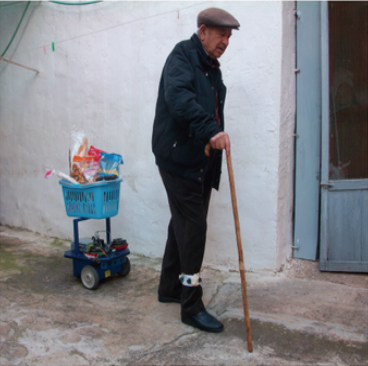
\includegraphics[width=0.4\textwidth]{figs/img/CompaRob}
   \caption{CompaRob Robot}
   \label{fig:CompaRob}
\end{figure}

\begin{figure}[b]
   \centering
   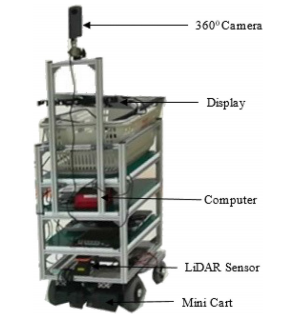
\includegraphics[width=0.38\textwidth]{figs/img/ShoppingSuportRobot}
   \caption{Shopping Support Robot}
   \label{fig:ShoppingSup}
\end{figure}

\begin{figure}[b]
   \centering
   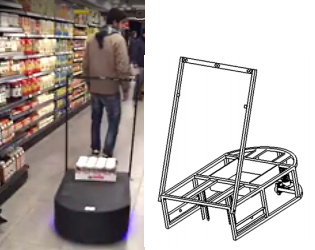
\includegraphics[width=0.45\textwidth]{figs/img/SmartCart}
   \caption{Smart Cart Robot}
   \label{fig:SmartCart}
\end{figure}

\vspace*{12pt}
\noindent
In the current project, we are implementing XBee S2C RF radios, which are inexpensive and easily configurable, as a remote target device that is carried by the user. The robot will be able to track this remote instead of using line of sight methods~\cite{Miah2018-Intelligent}. In addition to the XBee S2C RF radios, we will equip the robot with a parabolic reflector, which improves radio reception at various distances and angles, \textit{i.e.,} angle of arrivals of RF signals from the remote, based on research done previously in this type of robot localization and mapping~\cite{Miah2018-Intelligent}~\cite{Li2013ANA}.

\vspace*{12pt}
\noindent
The approach using signal strength of RF signals also requires an understanding of multipath interference which is common in RF based wireless positioning sensing systems. Authors in~\cite{xie_jiang_zhao_zhang_2019} explain that using course estimation calculations such as received signal strength indicator (RSSI) and time difference of arrival (TDoA) is key to compensate for the multipath interference in received signals.

\vspace*{12pt}
\noindent
The work in ~\cite{ladd_bekris_rudys_kavraki_wallach_2005} shows a different approach to the multipath issue by using an IEEE 802.11b wireless ethernet device to measure RF signals. This device system was used because it is communicable between a mobile device and a localization based service with low complexity for the user.

\vspace*{12pt}
\noindent
Also, in~\cite{lindhe_johansson_bicchi_2007}, the research states several other ways to counteract the multipath fading with methods such as antenna diversity, frequency spreading, or adaptive antenna arrays. The method used in this paper was to sample the radio signal strength (RSS) at discrete points without too much deviation from the robot's desired position in an indoor environment.

\vspace*{12pt}
\noindent
Lastly, in~\cite{Lindhe2009} the method that is utilized exploits multipath fading by measuring the signal-to-noise ratio (SNR) and adjusting the robot's motion to spend more time where the channel strength is greater.

\vspace*{12pt}
\noindent
All of the solutions that were found required line-of-sight communication between the robot and the user. In this project we aim to use the XBee S2C RF radios and a parabolic reflector combined into a rotating system similar to the one presented in~\cite{Miah2018-Intelligent} in order to have the robot track the customer through a store without using line-of-sight sensing. The major challenge of this implementation will be estimating the distance between the robot and the remote in varying environments.

%----------------------------------------------------------------------
\section{Report Organization}
%----------------------------------------------------------------------
\begin{itemize}
    \item Chapter \ref{ch: Chapter1} discusses the background and goals of the project and what other similar projects have accomplished.
    \item Chapter \ref{ch: Chapter2} explains how the robotic cart system in this project is broken down fundamentally, and the components used to build the robot.
    \item Chapter \ref{ch: Chapter3} goes over the design of the parabolic reflector arrays and how they were set up on the robot.
    \item Chapter \ref{ch: Chapter4} provides an explanation of the algorithms that were used to create the code to make the robot move.
    \item Chapter \ref{ch: Chapter5} discusses the implementation of all the parts onto the robot and the experimental results obtained when running the robot.
    \item Chapter \ref{ch: Chapter6} concludes the project work and discusses future endeavors on this project.
\end{itemize}

%%% Local Variables:
%%% mode: latex
%%% TeX-master: "../finalReport"
%%% End:
